\section{ROOMLanguage}
	The Real Time Object Oriented Modeling (ROOM).
	
	eTrice comprises several models:
	
	\begin{itemize}
	\item the ROOM model (*.room) -- defines model classes and the logical structure of the model
	\item the Config model (*.config) -- defines configuration values for attributes
	\item the Physical model (*.etphys) -- defines the structure and properties of the physical system
	\item the Mapping model (*.etmap) -- defines a mapping from logical elements to physical elements
	\end{itemize}
	
	In the following diagram the models and their relations are depicted. The meaning of the arrows is: uses/references.
	\begin{center}
		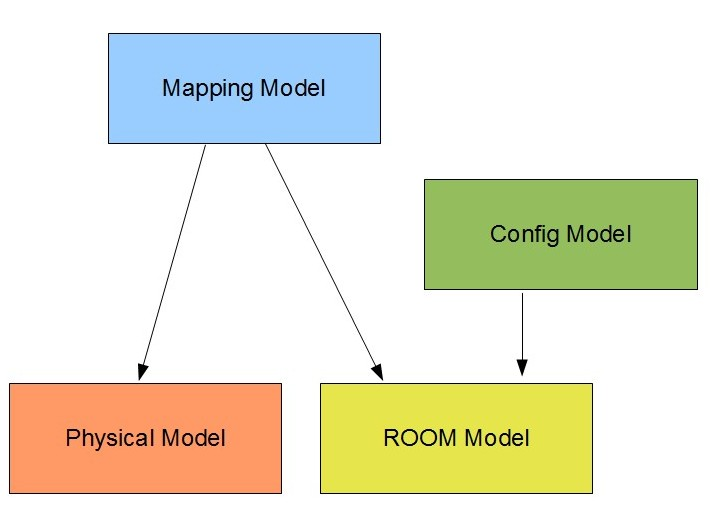
\includegraphics[width=.5\textwidth]{images/080-models.jpg}
	\end{center}
	
	\subsection{LogicalModel}
	The LogicalModel describes the logical structure and behavior of a ROOM application.
	
	The ROOM model defines DataTypes, ProtocolClasses, ActorClasses, SubSystemClasses and LogicalSystems.
	Thereby the three latter form a hierarchy. The LogicalSystem is the top level element of the structure. 
	It contains references to SubSystemClass elements. The SubSystemClass in turn contains 
	references to ActorClass elements which again contain (recursively) references to 
	ActorClass elements. The complete structural hierarchy implies a tree which has the 
	LogicalSystem as root and where each reference stands for a new node with possibly further 
	branches.
	
	\begingroup
	\textbf{Features:}
	%\setlength{\tabcolsep}{10pt} % Default value: 6pt
	\renewcommand{\arraystretch}{1.8} % Default value: 1
	\begin{longtable}{l|l p{.5\textwidth}}
		\hline
	Contains: & \tabitem \hyperlink{ref:LogicalSystem}{LogicalSystem}  & The top level structural class. It can only contain sub systems using SubSystemRefs.\\
	& \tabitem \hyperlink{ref:SubSystemClass}{SubSystemClass}  & The SubSystem is main Actor of an executable part of the system.  \\
	& \tabitem \hyperlink{ref:ActorClass}{ActorClass}  & The actor is the basic structural building block for building systems with ROOM. \\
	& \tabitem \hyperlink{ref:ProtocolClass}{ProtocolClass}  & A ProtocolClass defines messages and is the interface specification for a Port \\
	& \tabitem \hyperlink{ref:DataType}{DataType}  & A DataType can take 4 forms and types data elements like an Attribute or Operation argument. \\
	\hline
	\end{longtable}
	\endgroup
	
	
	\subsubsection{ActorClass}
		\hypertarget{ref:ActorClass}{}
		
		The actor is the basic structural building block for building systems with ROOM.
		
		An actor can be refined hierarchically and thus can be of arbitrarily large scope. Ports define the interface of an actor. An actor can also have a behavior usually defined by a finite state machine. 
		
		
		
		\begingroup
		\textbf{Features:}
		%\setlength{\tabcolsep}{10pt} % Default value: 6pt
		\renewcommand{\arraystretch}{1.8} % Default value: 1
		\begin{longtable}{l|l p{.5\textwidth}}
			\hline
		Contains: & \tabitem \hyperlink{ref:ExecutionType}{ExecutionType}  & Determines the execution type of an actor.\\
		& \tabitem \hyperlink{ref:ActorRef}{ActorRef}  & An ActorRef is an instance of an ActorClass. \\
		& \tabitem \hyperlink{ref:Port}{Port}  & A Port is an instance of a ProtocolClass and the interface for an ActorClass. \\
		& \tabitem \hyperlink{ref:SAP}{SAP}  & A Service Access Point is similar to a Port, but uses a LayerConnection for wiring. \\
		& \tabitem \hyperlink{ref:SPP}{SPP}  & A Service Provision Point is the counterpart of a SAP \\
		& \tabitem \hyperlink{ref:Binding}{Binding}  & A Binding connects two Ports with each other. \\
		& \tabitem \hyperlink{ref:LayerConnection}{LayerConnection}  & A LayerConnection associates a SPP to an ActorRef, resulting in an connection of all SAPs on its instance hierarchy. \\
		& \tabitem \hyperlink{ref:Attribute}{Attribute}  & An Attribute is a member variable of a class \\
		& \tabitem \hyperlink{ref:Operation}{Operation}  & An Operation is a member function of a class \\
		& \tabitem \hyperlink{ref:StateMachine}{StateMachine}  & A StateMachine describes the state based, event driven behavior of an ActorClass \\
		\hline
		Uses: & \tabitem \hyperlink{ref:Inheritance}{Inheritance}  & A class can specify a super class and inherits elements from the super class hierarchy.\\
		\hline
		\end{longtable}
		\endgroup
		
		\begingroup
		\textbf{Feature Usage:}
		%\setlength{\tabcolsep}{10pt} % Default value: 6pt
		\renewcommand{\arraystretch}{1.8} % Default value: 1
		\begin{longtable}{l|l p{.5\textwidth}}
			\hline
		Typecasts: & \tabitem \hyperlink{ref:ActorRef}{ActorRef}  & An ActorRef is an instance of an ActorClass.\\
		\hline
		Is contained in: & \tabitem \hyperlink{ref:LogicalModel}{LogicalModel}  & The LogicalModel describes the logical structure and behavior of a ROOM application.\\
		\hline
		Is edited by: & \tabitem \hyperlink{ref:GraphicalStructureEditor}{GraphicalStructureEditor}  & The Structure Editor allows to edit the Actor Structure in a convenient way. It is possible to create and arrange actor references and ports and to create bindings and layer connections.\\
		\hline
		\end{longtable}
		\endgroup
		
		\textbf{Example:}
		
			
	
	\vspace{\baselineskip}
	\vspace{\baselineskip}
	\vspace{\baselineskip}
	
	\subsubsection{ActorRef}
		\hypertarget{ref:ActorRef}{}
		
		An ActorRef is an instance of an ActorClass.
		
		
		\textbf{Properties:}
		\begin{itemize}
		\item multiplicity : '\verb|1..n|', '\verb|*|'
		\end{itemize}
		
		\begingroup
		\textbf{Features:}
		%\setlength{\tabcolsep}{10pt} % Default value: 6pt
		\renewcommand{\arraystretch}{1.8} % Default value: 1
		\begin{longtable}{l|l p{.5\textwidth}}
			\hline
		Is of type: & \tabitem \hyperlink{ref:ActorClass}{ActorClass}  & The actor is the basic structural building block for building systems with ROOM.\\
		\hline
		\end{longtable}
		\endgroup
		
		\begingroup
		\textbf{Feature Usage:}
		%\setlength{\tabcolsep}{10pt} % Default value: 6pt
		\renewcommand{\arraystretch}{1.8} % Default value: 1
		\begin{longtable}{l|l p{.5\textwidth}}
			\hline
		Is contained in: & \tabitem \hyperlink{ref:ActorClass}{ActorClass}  & The actor is the basic structural building block for building systems with ROOM.\\
		& \tabitem \hyperlink{ref:SubSystemClass}{SubSystemClass}  & The SubSystem is main Actor of an executable part of the system.  \\
		\hline
		Is edited by: & \tabitem \hyperlink{ref:ActorRefPropertyDialog}{ActorRefPropertyDialog}  & A Dialog to edit structural reference of an ActorRef.
		\\
		& \tabitem \hyperlink{ref:GraphicalStructureEditor}{GraphicalStructureEditor}  & The Structure Editor allows to edit the Actor Structure in a convenient way. It is possible to create and arrange actor references and ports and to create bindings and layer connections. \\
		\hline
		\end{longtable}
		\endgroup
		
		\textbf{Example:}
		
			\begin{lstlisting}[language=ROOM]
			SubSystemClass SubSystemExample {
				ActorRef mainActor : ActorClassExample
				
				LogicalThread default_thread
			}
			
			ActorClass ActorClassExample {
				Structure {
					ActorRef sender : Sender
					ActorRef receiver : Receiver
					
					Binding receiver.port and sender.port
				}
			}
			
			ActorClass ActorClassExampleReplicated {
				Structure {
					ActorRef sender[3]: Sender
					ActorRef receiver[3] : Receiver
					
					Binding receiver.port and sender.port
					/* Equivalent to:
					 *  Binding receiver[1].port and sender[1].port
					 *  Binding receiver[2].port and sender[2].port
					 * ....
					 */		
				}
			}
			\end{lstlisting}
			\begin{figure}[H]
			\includegraphics[width=.7\textwidth]{images/300-ActorRefInstanceDiagram.jpg}
			\caption*{Instance hierarchy of ActorRef Example (\textsf{System(System)} not shown in code snippet)}
			\end{figure}
	
	\vspace{\baselineskip}
	\vspace{\baselineskip}
	\vspace{\baselineskip}
	
	\subsubsection{Attribute}
		\hypertarget{ref:Attribute}{}
		
		An Attribute is a member variable of a class
		
		An Attribute can be be used to store arbitrary data. There are two common conceptual purpose of use:
		\begin{itemize}
			\item model stateful behavior (extended state machine variable)
			\item store reference to more fine-grained components (e.g. c pointer to handle)
		\end{itemize}
		Attributes can be defined in ActorClasses, DataClasses and ProtocolClasses.
		
		\textbf{Properties:}
		\begin{itemize}
		\item defaultValueLiteral : '\verb|<target code>|'
		\item multiplicity : '\verb|1..n|'
		\end{itemize}
		
		\begingroup
		\textbf{Features:}
		%\setlength{\tabcolsep}{10pt} % Default value: 6pt
		\renewcommand{\arraystretch}{1.8} % Default value: 1
		\begin{longtable}{l|l p{.5\textwidth}}
			\hline
		Is of type: & \tabitem \hyperlink{ref:DataType}{DataType}  & A DataType can take 4 forms and types data elements like an Attribute or Operation argument.\\
		\hline
		\end{longtable}
		\endgroup
		
		\begingroup
		\textbf{Feature Usage:}
		%\setlength{\tabcolsep}{10pt} % Default value: 6pt
		\renewcommand{\arraystretch}{1.8} % Default value: 1
		\begin{longtable}{l|l p{.5\textwidth}}
			\hline
		Is contained in: & \tabitem \hyperlink{ref:ActorClass}{ActorClass}  & The actor is the basic structural building block for building systems with ROOM.\\
		& \tabitem \hyperlink{ref:DataClass}{DataClass}  & A DataClass is a composition of Attributes. \\
		& \tabitem \hyperlink{ref:ProtocolClass}{ProtocolClass}  & A ProtocolClass defines messages and is the interface specification for a Port \\
		\hline
		\end{longtable}
		\endgroup
		
		\textbf{Example:}
		
				\begin{lstlisting}[language=ROOM]
				import room.basic.types.* from "../../../org.eclipse.etrice.modellib.c/model/Types.room"
				
				DataClass SimpleDataClass {
					Attribute attribute1: int16
					Attribute attribute2: uint32
				}
			
				ActorClass ActorClassWithAttributes {
					Structure {
						Attribute attribute1: int32 			["attribute of a PrimitiveType" ]
						Attribute attribute2: SimpleDataClass 	[ "attribute of a DataClass" ]
					}
				}
			
				ActorClass ActorClassWithAttributes2 {
					Structure {
						Attribute arrayAttribute[8] : uint32 [ "attribute with multiplicity"]
						Attribute refAttribue : voidType ref [ "attribute as a reference (void pointer)"]
					}
				}
			
				ActorClass ActorClassWithAttributeInitialization {
					Structure {
						Attribute attribute1: uint32 = "3"
						Attribute attribute2: SimpleDataClass = "{1, 2}"
						Attribute arrayAttribute[8] : uint32 = "0" // or {0,0,0, ...}
						Attribute refAttribue : voidType ref = "NULL" // set reference in constructor or in state machine
					}
				}
				\end{lstlisting}
	
	\vspace{\baselineskip}
	\vspace{\baselineskip}
	\vspace{\baselineskip}
	
	\subsubsection{Binding}
		\hypertarget{ref:Binding}{}
		
		A Binding connects two Ports with each other.
		
		
		
		\begingroup
		\textbf{Features:}
		%\setlength{\tabcolsep}{10pt} % Default value: 6pt
		\renewcommand{\arraystretch}{1.8} % Default value: 1
		\begin{longtable}{l|l p{.5\textwidth}}
			\hline
		Uses: & \tabitem \hyperlink{ref:Port}{Port} : endpoint1 & A Port is an instance of a ProtocolClass and the interface for an ActorClass.\\
		& \tabitem \hyperlink{ref:Port}{Port} : endpoint2 & A Port is an instance of a ProtocolClass and the interface for an ActorClass. \\
		\hline
		\end{longtable}
		\endgroup
		
		\begingroup
		\textbf{Feature Usage:}
		%\setlength{\tabcolsep}{10pt} % Default value: 6pt
		\renewcommand{\arraystretch}{1.8} % Default value: 1
		\begin{longtable}{l|l p{.5\textwidth}}
			\hline
		Is contained in: & \tabitem \hyperlink{ref:ActorClass}{ActorClass}  & The actor is the basic structural building block for building systems with ROOM.\\
		& \tabitem \hyperlink{ref:LogicalSystem}{LogicalSystem}  & The top level structural class. It can only contain sub systems using SubSystemRefs. \\
		& \tabitem \hyperlink{ref:SubSystemClass}{SubSystemClass}  & The SubSystem is main Actor of an executable part of the system.  \\
		\hline
		Is edited by: & \tabitem \hyperlink{ref:GraphicalStructureEditor}{GraphicalStructureEditor}  & The Structure Editor allows to edit the Actor Structure in a convenient way. It is possible to create and arrange actor references and ports and to create bindings and layer connections.\\
		\hline
		\end{longtable}
		\endgroup
		
		
	\vspace{\baselineskip}
	\vspace{\baselineskip}
	\vspace{\baselineskip}
	
	\subsubsection{CommunicationType}
		\hypertarget{ref:CommunicationType}{}
		
		The CommunicationType defines the communication semantics of a ProtocolClass.
		
		Since from ROOM models executable code can be generated, it is important to define the way the actors are 
		executed and communicate with each other. The combination of communication and execution is called the 
		\emph{execution model}. Therefore the ExecutionType of an actor and the CommunicationType of the ports has to be considered.
		
		The CommunicationType of a ProtocolClass (and thus of a Port) specifies in which way the communication should happen:
		
		\begin{itemize}
		\item \textbf{message driven} -- asynchronous, non blocking, no return value:\\
		Usually the message driven communication is implemented with message queues. Message queues are inherently asynchronous and enable a very good decoupling of the communicating parties.
		\item \textbf{data driven} -- asynchronous, non blocking, no return value:\\
		In data driven communication sender and receiver often have a shared block of data. The sender writes the data and the receiver polls the data.
		\item \textit{\textbf{function call} -- synchronous, blocking, return value:\\
		Regular function call as known in most programming languages.} (not supported yet)
		\end{itemize}
		
		CommunicationType relates with the \hyperlink{ref:ExecutionType}{ExecutionType} of an ActorClass, e.g. a data-driven port needs a cyclic thread, that polls the shared data.
		
		\textbf{Properties:}
		\begin{itemize}
		\item type : '\verb|eventdriven|', '\verb|datadriven|', '\verb|sync|'
		\end{itemize}
		
		
		\begingroup
		\textbf{Feature Usage:}
		%\setlength{\tabcolsep}{10pt} % Default value: 6pt
		\renewcommand{\arraystretch}{1.8} % Default value: 1
		\begin{longtable}{l|l p{.5\textwidth}}
			\hline
		Is contained in: & \tabitem \hyperlink{ref:ProtocolClass}{ProtocolClass}  & A ProtocolClass defines messages and is the interface specification for a Port\\
		\hline
		Is used by: & \tabitem \hyperlink{ref:ExecutionType}{ExecutionType}  & Determines the execution type of an actor.\\
		\hline
		\end{longtable}
		\endgroup
		
		\textbf{Example:}
		
				\begin{lstlisting}[language=ROOM]
			
				import room.basic.types.* from "../../../org.eclipse.etrice.modellib.c/model/Types.room"
			
				ProtocolClass EventdrivenProtocolClass1 [ "default is eventdriven" ] {
					// explicit: eventdriven ProtocolClass EventdrivenProtocolClass {
					incoming {
						Message msg1() ["message without data"]
						Message msg2(data: int32) ["message with data"]
					}
					outgoing {
						Message msg4()  ["eventdriven ProtocolClass can have message into two directions"]
					}
				}
			
				datadriven ProtocolClass DatadrivenProtocolClass {
					incoming {
						Message signal1 (data: int32) ["a datadriven message needs data"]
					}
					// datadriven ProtocolClass can only have incoming messages (signals)
				}
				
				//  sync is not supported yet
				//	sync ProtocolClass SyncProtcolClass { 
				//		
				//	}
				\end{lstlisting}
	
	\vspace{\baselineskip}
	\vspace{\baselineskip}
	\vspace{\baselineskip}
	
	\subsubsection{DataClass}
		\hypertarget{ref:DataClass}{}
		
		A DataClass is a composition of Attributes.
		
		Intended to model a type that primarily consists of data, which is usually grouped together in some manner. DataClasses roughly translate to Java classes without interaction or C \textsf{struct}s.
		
		\begin{lstlisting}[language=ROOM]		
		DataClass TCPConnectionData {
			Attribute IPAddr: string
			Attribute TcpPort: int32
		}
		\end{lstlisting}
		
		
		\begingroup
		\textbf{Features:}
		%\setlength{\tabcolsep}{10pt} % Default value: 6pt
		\renewcommand{\arraystretch}{1.8} % Default value: 1
		\begin{longtable}{l|l p{.5\textwidth}}
			\hline
		Is a: & \tabitem \hyperlink{ref:DataType}{DataType}  & A DataType can take 4 forms and types data elements like an Attribute or Operation argument.\\
		\hline
		Contains: & \tabitem \hyperlink{ref:Attribute}{Attribute}  & An Attribute is a member variable of a class\\
		& \tabitem \hyperlink{ref:Operation}{Operation}  & An Operation is a member function of a class \\
		\hline
		Uses: & \tabitem \hyperlink{ref:Inheritance}{Inheritance}  & A class can specify a super class and inherits elements from the super class hierarchy.\\
		\hline
		\end{longtable}
		\endgroup
		
		
		\textbf{Example:}
		
			\begin{lstlisting}[language=ROOM]
			DataClass SimpleDataClass {
				Attribute attribute1: uint16
				Attribute attribute2: uint32
			}
			
			DataClass DataClassExample {
				Attribute attribute1: uint32
				Attribute attribute2: SimpleDataClass
				Attribute attribute3: voidType ref
				
				Operation operation1(param1: uint32, param2: uint16): boolean {
					"return true;"
				}
			}
			\end{lstlisting}
	
	\vspace{\baselineskip}
	\vspace{\baselineskip}
	\vspace{\baselineskip}
	
	\subsubsection{DataType}
		\hypertarget{ref:DataType}{}
		
		A DataType can take 4 forms and types data elements like an Attribute or Operation argument.
		
		
		
		
		\begingroup
		\textbf{Feature Usage:}
		%\setlength{\tabcolsep}{10pt} % Default value: 6pt
		\renewcommand{\arraystretch}{1.8} % Default value: 1
		\begin{longtable}{l|l p{.5\textwidth}}
			\hline
		Inheriting features: & \tabitem \hyperlink{ref:DataClass}{DataClass}  & A DataClass is a composition of Attributes.\\
		& \tabitem \hyperlink{ref:EnumerationType}{EnumerationType}  & An EnumerationType declares an enumeration similar to most well-known languages. \\
		& \tabitem \hyperlink{ref:ExternalType}{ExternalType}  & An ExternalType is used to make an target language type accessible in ROOM. \\
		& \tabitem \hyperlink{ref:PrimitiveType}{PrimitiveType}  & A PrimitiveType is an abstraction of a target language's basic type (e.g. integer or boolean). \\
		\hline
		Typecasts: & \tabitem \hyperlink{ref:Attribute}{Attribute}  & An Attribute is a member variable of a class\\
		\hline
		Is contained in: & \tabitem \hyperlink{ref:LogicalModel}{LogicalModel}  & The LogicalModel describes the logical structure and behavior of a ROOM application.\\
		\hline
		Is used by: & \tabitem \hyperlink{ref:Operation}{Operation}  & An Operation is a member function of a class\\
		\hline
		\end{longtable}
		\endgroup
		
		
	\vspace{\baselineskip}
	\vspace{\baselineskip}
	\vspace{\baselineskip}
	
	\subsubsection{EnumerationType}
		\hypertarget{ref:EnumerationType}{}
		
		An EnumerationType declares an enumeration similar to most well-known languages.
		
		
		\textbf{Properties:}
		\begin{itemize}
		\item literals : '\verb|<name>|'
		\end{itemize}
		
		\begingroup
		\textbf{Features:}
		%\setlength{\tabcolsep}{10pt} % Default value: 6pt
		\renewcommand{\arraystretch}{1.8} % Default value: 1
		\begin{longtable}{l|l p{.5\textwidth}}
			\hline
		Is a: & \tabitem \hyperlink{ref:DataType}{DataType}  & A DataType can take 4 forms and types data elements like an Attribute or Operation argument.\\
		\hline
		\end{longtable}
		\endgroup
		
		
		\textbf{Example:}
		
			\begin{lstlisting}[language=ROOM]
			Enumeration EOnOff {
				Off = 0, // explicit value=0
				On = 1 // explicit value=1 
			
			}
			
			Enumeration EDay {
				SUN,
				MON,
				TUE,
				WED,
				THU,
				FRI,
				SAT // implicit enumeration 0..6
			}
			\end{lstlisting}
	
	\vspace{\baselineskip}
	\vspace{\baselineskip}
	\vspace{\baselineskip}
	
	\subsubsection{ExecutionType}
		\hypertarget{ref:ExecutionType}{}
		
		Determines the execution type of an actor.
		
		Since from ROOM models executable code can be generated, it is important to define the way the actors are 
		executed and communicate with each other. The combination of communication and execution is called the 
		\emph{execution model}. Therefore the ExecutionType of an actor and the CommunicationType of the ports has to be considered.
		
		The ExecutionType of an ActorClass specifies in which way its instance (ActorRef) should be executed:
		\begin{itemize}
		\item \textbf{execution by receive event}: The message queue or the event dispatcher calls a 
		\textbf{receive event} function of the message receiver and thereby executes the processing of the event.
		\item \textbf{polled execution}: The objects are processed by a cyclic \textbf{execute} call
		\item \textit{\textbf{execution by function call}: The caller executes the called object via function call} (not supported yet)
		\item \textbf{mixture}: An asynchronous execution combines an event dispachter and a polled execution.
		\end{itemize}
		
		Thereby the ExecutionType determines the execution mode of the actor's logical thread:
		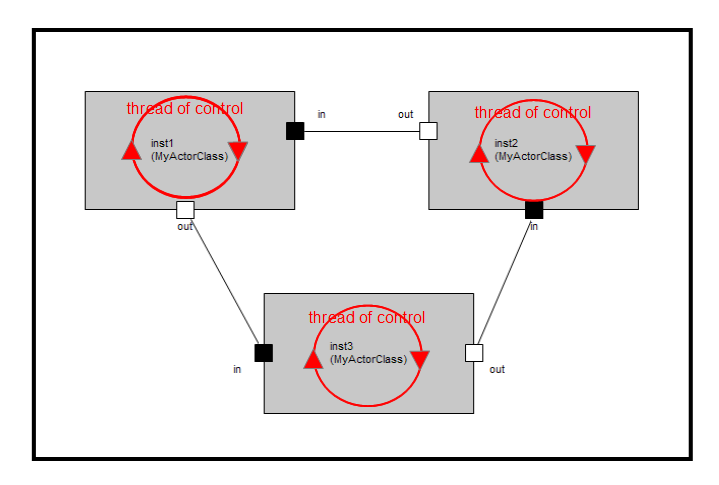
\includegraphics[width=.7\textwidth]{images/010-RoomIntroduction03.png}
				
		The actual execution of the underlying physical thread can be specified in the PhysicalModel in conjunction with the MappingModel.
		
		ExecutionType relates to the \hyperlink{ref:CommunicationType}{CommunicationType}, e.g. if an actor uses data-driven ports, it should support an polled execution.
		
		\textbf{Properties:}
		\begin{itemize}
		\item mode : '\verb|eventdriven|', '\verb|datadriven|', '\verb|async|', '\verb|sync|'
		\end{itemize}
		
		\begingroup
		\textbf{Features:}
		%\setlength{\tabcolsep}{10pt} % Default value: 6pt
		\renewcommand{\arraystretch}{1.8} % Default value: 1
		\begin{longtable}{l|l p{.5\textwidth}}
			\hline
		Uses: & \tabitem \hyperlink{ref:CommunicationType}{CommunicationType}  & The CommunicationType defines the communication semantics of a ProtocolClass.\\
		\hline
		\end{longtable}
		\endgroup
		
		\begingroup
		\textbf{Feature Usage:}
		%\setlength{\tabcolsep}{10pt} % Default value: 6pt
		\renewcommand{\arraystretch}{1.8} % Default value: 1
		\begin{longtable}{l|l p{.5\textwidth}}
			\hline
		Is contained in: & \tabitem \hyperlink{ref:ActorClass}{ActorClass}  & The actor is the basic structural building block for building systems with ROOM.\\
		\hline
		\end{longtable}
		\endgroup
		
		\textbf{Example:}
		
			\begin{lstlisting}
			eventdriven ActorClass EventdrivenActor ["default is eventdriven"] {
				// only event-driven Ports and ActorRefs allowed
			}
			
			datadriven ActorClass DatadrivenActor {
				// only data-driven Ports and ActorRefs allowed
			}
			
			async ActorClass MixedActor{
				// both data/event-driven Ports and ActorRefs allowed
			}
			\end{lstlisting}
	
	\vspace{\baselineskip}
	\vspace{\baselineskip}
	\vspace{\baselineskip}
	
	\subsubsection{ExternalEndPort}
		\hypertarget{ref:ExternalEndPort}{}
		
		A ExternalEndPort is an interface Port, that is made accessible to the internal interface of an ActorClass.
		
		\begin{lstlisting}[language=ROOM]
		ActorClass ExternalEndPortExample {
			Interface {
				// externalEndPort is connect from 'outside' and thus needs a Binding from containing ActorClass
				Port externalEndPort : PSimpleProtocol
			}
			Structure {
				external Port externalEndPort
			}
			Behavior {
				// send/receive messages from externalEndPort
			}
		}
		\end{lstlisting}
		
		
		\begingroup
		\textbf{Features:}
		%\setlength{\tabcolsep}{10pt} % Default value: 6pt
		\renewcommand{\arraystretch}{1.8} % Default value: 1
		\begin{longtable}{l|l p{.5\textwidth}}
			\hline
		Is a: & \tabitem \hyperlink{ref:Port}{Port}  & A Port is an instance of a ProtocolClass and the interface for an ActorClass.\\
		\hline
		\end{longtable}
		\endgroup
		
		
		
	\vspace{\baselineskip}
	\vspace{\baselineskip}
	\vspace{\baselineskip}
	
	\subsubsection{ExternalType}
		\hypertarget{ref:ExternalType}{}
		
		An ExternalType is used to make an target language type accessible in ROOM.
		
		
		\textbf{Properties:}
		\begin{itemize}
		\item targetName : '\verb|<identifier name>|'
		\end{itemize}
		
		\begingroup
		\textbf{Features:}
		%\setlength{\tabcolsep}{10pt} % Default value: 6pt
		\renewcommand{\arraystretch}{1.8} % Default value: 1
		\begin{longtable}{l|l p{.5\textwidth}}
			\hline
		Is a: & \tabitem \hyperlink{ref:DataType}{DataType}  & A DataType can take 4 forms and types data elements like an Attribute or Operation argument.\\
		\hline
		\end{longtable}
		\endgroup
		
		
		\textbf{Example:}
		
			\begin{lstlisting}[language=ROOM]
			// Include is needed when used (e.g. in ActorClassWithExternalType)
			ExternalType someStructType -> "struct FILE_HANDLE"
			
			ActorClass ActorClassWithExternalType{
				Structure {
					usercode1 {
						"// #include <___.h> /* User includes here*/"
					}
					Attribute someHandle : someStructType ref // needs include
				}
				Behavior {
					Operation operation1(param1: charPtr) {
						// external calls or casts may need includes
						"write(someHandle, param1);"
					}
				}
			}
			\end{lstlisting}
	
	\vspace{\baselineskip}
	\vspace{\baselineskip}
	\vspace{\baselineskip}
	
	\subsubsection{InternalEndPort}
		\hypertarget{ref:InternalEndPort}{}
		
		A InternalEndPort is an local Port, that is declared in the internal interface of an ActorClass.
		
		\begin{lstlisting}[language=ROOM]
		ActorClass InternalEndPortExample {
			Structure {
				Port internalEndPort : PSimpleProtocol
				ActorRef actorRef1 : SimpleActorClass
				
				// internalEndPort lives 'local' and
				// thus needs a Binding to port of a ActorRef
				Binding internalEndPort and actorRef1.externalPort2 
			}
			Behavior {
				// send/receive messages from internalEndPorts
			}
		}
		\end{lstlisting}
		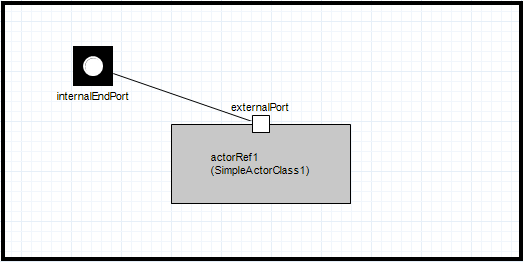
\includegraphics[scale=.7]{images/300-InternalEndPort.png}
		
		
		\begingroup
		\textbf{Features:}
		%\setlength{\tabcolsep}{10pt} % Default value: 6pt
		\renewcommand{\arraystretch}{1.8} % Default value: 1
		\begin{longtable}{l|l p{.5\textwidth}}
			\hline
		Is a: & \tabitem \hyperlink{ref:Port}{Port}  & A Port is an instance of a ProtocolClass and the interface for an ActorClass.\\
		\hline
		\end{longtable}
		\endgroup
		
		
		
	\vspace{\baselineskip}
	\vspace{\baselineskip}
	\vspace{\baselineskip}
	
	\subsubsection{LayerConnection}
		\hypertarget{ref:LayerConnection}{}
		
		A LayerConnection associates a SPP to an ActorRef, resulting in an connection of all SAPs on its instance hierarchy.
		
		\begin{itemize}
		\item An actor class can define a Service Provision Point (SPP) to publish a specific service, defined by a protocol class
		\item An actor class can define a Service Access Point (SAP) if it needs a service, defined by a protocol class
		\item For a given actor hierarchy, a LayerConnection defines which SAP will be satisfied by (connected to) which SPP
		\end{itemize}
		
		
		\begingroup
		\textbf{Features:}
		%\setlength{\tabcolsep}{10pt} % Default value: 6pt
		\renewcommand{\arraystretch}{1.8} % Default value: 1
		\begin{longtable}{l|l p{.5\textwidth}}
			\hline
		Uses: & \tabitem \hyperlink{ref:SAP}{SAP} : SAPoint & A Service Access Point is similar to a Port, but uses a LayerConnection for wiring.\\
		& \tabitem \hyperlink{ref:SPP}{SPP} : SPPoint & A Service Provision Point is the counterpart of a SAP \\
		\hline
		\end{longtable}
		\endgroup
		
		\begingroup
		\textbf{Feature Usage:}
		%\setlength{\tabcolsep}{10pt} % Default value: 6pt
		\renewcommand{\arraystretch}{1.8} % Default value: 1
		\begin{longtable}{l|l p{.5\textwidth}}
			\hline
		Is contained in: & \tabitem \hyperlink{ref:ActorClass}{ActorClass}  & The actor is the basic structural building block for building systems with ROOM.\\
		& \tabitem \hyperlink{ref:LogicalSystem}{LogicalSystem}  & The top level structural class. It can only contain sub systems using SubSystemRefs. \\
		& \tabitem \hyperlink{ref:SubSystemClass}{SubSystemClass}  & The SubSystem is main Actor of an executable part of the system.  \\
		\hline
		Is edited by: & \tabitem \hyperlink{ref:GraphicalStructureEditor}{GraphicalStructureEditor}  & The Structure Editor allows to edit the Actor Structure in a convenient way. It is possible to create and arrange actor references and ports and to create bindings and layer connections.\\
		\hline
		\end{longtable}
		\endgroup
		
		
	\vspace{\baselineskip}
	\vspace{\baselineskip}
	\vspace{\baselineskip}
	
	\subsubsection{LogicalSystem}
		\hypertarget{ref:LogicalSystem}{}
		
		The top level structural class. It can only contain sub systems using SubSystemRefs.
		
		The LogicalSystem is composed of sub system instances. It also defines Bindings and LayerConnections between those sub systems. 
		
		
		\begingroup
		\textbf{Features:}
		%\setlength{\tabcolsep}{10pt} % Default value: 6pt
		\renewcommand{\arraystretch}{1.8} % Default value: 1
		\begin{longtable}{l|l p{.5\textwidth}}
			\hline
		Contains: & \tabitem \hyperlink{ref:SubSystemRef}{SubSystemRef}  & A Sub System Reference is an instance of an SubSystemClass\\
		& \tabitem \hyperlink{ref:Binding}{Binding}  & A Binding connects two Ports with each other. \\
		& \tabitem \hyperlink{ref:LayerConnection}{LayerConnection}  & A LayerConnection associates a SPP to an ActorRef, resulting in an connection of all SAPs on its instance hierarchy. \\
		\hline
		\end{longtable}
		\endgroup
		
		\begingroup
		\textbf{Feature Usage:}
		%\setlength{\tabcolsep}{10pt} % Default value: 6pt
		\renewcommand{\arraystretch}{1.8} % Default value: 1
		\begin{longtable}{l|l p{.5\textwidth}}
			\hline
		Is contained in: & \tabitem \hyperlink{ref:LogicalModel}{LogicalModel}  & The LogicalModel describes the logical structure and behavior of a ROOM application.\\
		\hline
		\end{longtable}
		\endgroup
		
		
	\vspace{\baselineskip}
	\vspace{\baselineskip}
	\vspace{\baselineskip}
	
	\subsubsection{Operation}
		\hypertarget{ref:Operation}{}
		
		An Operation is a member function of a class
		
		
		\textbf{Properties:}
		\begin{itemize}
		\item returnType : '\verb|<DataType>|'
		\item arguments : '\verb|<name> : <DataType>|'
		\end{itemize}
		
		\begingroup
		\textbf{Features:}
		%\setlength{\tabcolsep}{10pt} % Default value: 6pt
		\renewcommand{\arraystretch}{1.8} % Default value: 1
		\begin{longtable}{l|l p{.5\textwidth}}
			\hline
		Uses: & \tabitem \hyperlink{ref:DataType}{DataType}  & A DataType can take 4 forms and types data elements like an Attribute or Operation argument.\\
		\hline
		\end{longtable}
		\endgroup
		
		\begingroup
		\textbf{Feature Usage:}
		%\setlength{\tabcolsep}{10pt} % Default value: 6pt
		\renewcommand{\arraystretch}{1.8} % Default value: 1
		\begin{longtable}{l|l p{.5\textwidth}}
			\hline
		Is contained in: & \tabitem \hyperlink{ref:ActorClass}{ActorClass}  & The actor is the basic structural building block for building systems with ROOM.\\
		& \tabitem \hyperlink{ref:DataClass}{DataClass}  & A DataClass is a composition of Attributes. \\
		& \tabitem \hyperlink{ref:ProtocolClass}{ProtocolClass}  & A ProtocolClass defines messages and is the interface specification for a Port \\
		\hline
		\end{longtable}
		\endgroup
		
		\textbf{Example:}
		
				\begin{lstlisting}[language=ROOM]
				import room.basic.types.* from "../../../org.eclipse.etrice.modellib.c/model/Types.room"
			
				DataClass DataClassWithOperation {
					Attribute attribute1 : uint32
					
					Operation operation1(param1: uint32, param2: int32): boolean {
						"return attribute1 > (param1 - param2);"
					}
				}
				
				ActorClass ActorClassWithOperation {
					Structure {
						Attribute attribute1 : uint32
					}
					Behavior {
						Operation operation1(param1: uint32, param2: int32): boolean {
							"return attribute1 > (param1 - param2);"
						}
					}
				}
				
				ActorClass ActorClassWithOperation2 {
					Structure {
						usercode1 {
							"// #include <___.h> /* User includes here*/"
						}
						Attribute someHandle : voidType ref
					}
					Behavior {
						Operation operation1(param1: charPtr) {
							// external calls or casts may need includes
							"write(someHandle, param1);"
						}
					}
				}
				\end{lstlisting}
	
	\vspace{\baselineskip}
	\vspace{\baselineskip}
	\vspace{\baselineskip}
	
	\subsubsection{Port}
		\hypertarget{ref:Port}{}
		
		A Port is an instance of a ProtocolClass and the interface for an ActorClass.
		
		It provides strong decoupling of ActorClasses from each other, thus enabling easy testability, reusability and deployment of Actors to different threads or nodes.description
		
		\textbf{Properties:}
		\begin{itemize}
		\item conjugated : '\verb|regular|', '\verb|conjugated|'
		\item multiplicity : '\verb|1..n|', '\verb|*|'
		\end{itemize}
		
		\begingroup
		\textbf{Features:}
		%\setlength{\tabcolsep}{10pt} % Default value: 6pt
		\renewcommand{\arraystretch}{1.8} % Default value: 1
		\begin{longtable}{l|l p{.5\textwidth}}
			\hline
		Is of type: & \tabitem \hyperlink{ref:ProtocolClass}{ProtocolClass}  & A ProtocolClass defines messages and is the interface specification for a Port\\
		\hline
		\end{longtable}
		\endgroup
		
		\begingroup
		\textbf{Feature Usage:}
		%\setlength{\tabcolsep}{10pt} % Default value: 6pt
		\renewcommand{\arraystretch}{1.8} % Default value: 1
		\begin{longtable}{l|l p{.5\textwidth}}
			\hline
		Inheriting features: & \tabitem \hyperlink{ref:ExternalEndPort}{ExternalEndPort}  & A ExternalEndPort is an interface Port, that is made accessible to the internal interface of an ActorClass.\\
		& \tabitem \hyperlink{ref:InternalEndPort}{InternalEndPort}  & A InternalEndPort is an local Port, that is declared in the internal interface of an ActorClass. \\
		& \tabitem \hyperlink{ref:RelayPort}{RelayPort}  & A RelayPort forwards its messages without exposing them to the internal interface of the ActorClass. \\
		\hline
		Is contained in: & \tabitem \hyperlink{ref:ActorClass}{ActorClass}  & The actor is the basic structural building block for building systems with ROOM.\\
		\hline
		Is edited by: & \tabitem \hyperlink{ref:GraphicalStructureEditor}{GraphicalStructureEditor}  & The Structure Editor allows to edit the Actor Structure in a convenient way. It is possible to create and arrange actor references and ports and to create bindings and layer connections.\\
		& \tabitem \hyperlink{ref:PortPropertyDialog}{PortPropertyDialog}  &  \\
		\hline
		Is used by: & \tabitem \hyperlink{ref:Binding}{Binding} : endpoint1 & A Binding connects two Ports with each other.\\
		& \tabitem \hyperlink{ref:Binding}{Binding} : endpoint2 & A Binding connects two Ports with each other. \\
		\hline
		\end{longtable}
		\endgroup
		
		
	\vspace{\baselineskip}
	\vspace{\baselineskip}
	\vspace{\baselineskip}
	
	\subsubsection{PrimitiveType}
		\hypertarget{ref:PrimitiveType}{}
		
		A PrimitiveType is an abstraction of a target language's basic type (e.g. integer or boolean).
		
		
		\textbf{Properties:}
		\begin{itemize}
		\item targetName : '\verb|<identifer name>|'
		\end{itemize}
		
		\begingroup
		\textbf{Features:}
		%\setlength{\tabcolsep}{10pt} % Default value: 6pt
		\renewcommand{\arraystretch}{1.8} % Default value: 1
		\begin{longtable}{l|l p{.5\textwidth}}
			\hline
		Is a: & \tabitem \hyperlink{ref:DataType}{DataType}  & A DataType can take 4 forms and types data elements like an Attribute or Operation argument.\\
		\hline
		\end{longtable}
		\endgroup
		
		
		\textbf{Example:}
		
			The eTrice built-in types can be found in the \textsf{org.eclipse.etrice.modellib} project. In most cases the \textsf{Types.room} is already included:
			\begin{lstlisting}[language=ROOM]
			// Follow import by Open Declaration (F3)
			import room.basic.types.* from "../../../org.eclipse.etrice.modellib.c/model/Types.room"
			\end{lstlisting}
	
	\vspace{\baselineskip}
	\vspace{\baselineskip}
	\vspace{\baselineskip}
	
	\subsubsection{ProtocolClass}
		\hypertarget{ref:ProtocolClass}{}
		
		A ProtocolClass defines messages and is the interface specification for a Port
		
		A ProtocolClass provides a reusable interface specification for ports. It defines a set of incoming and outgoing Messages that can be exchanged between two ports.
		The exact semantics of a message is defined by the CommunicationType.
		Protocol classes have only textual notation.
		
		\begin{lstlisting}
		ProtocolClass SimpleProtocolClass {
			incoming {
				Message msg1(data: int32}
				Message msg2()
			}
			outgoing {
				Message msg3(data: DataClass1}
				Message msg4()
			}
		}
		\end{lstlisting}
		
		
		\begingroup
		\textbf{Features:}
		%\setlength{\tabcolsep}{10pt} % Default value: 6pt
		\renewcommand{\arraystretch}{1.8} % Default value: 1
		\begin{longtable}{l|l p{.5\textwidth}}
			\hline
		Contains: & \tabitem \hyperlink{ref:CommunicationType}{CommunicationType}  & The CommunicationType defines the communication semantics of a ProtocolClass.\\
		& \tabitem \hyperlink{ref:Attribute}{Attribute}  & An Attribute is a member variable of a class \\
		& \tabitem \hyperlink{ref:Operation}{Operation}  & An Operation is a member function of a class \\
		\hline
		Uses: & \tabitem \hyperlink{ref:Inheritance}{Inheritance}  & A class can specify a super class and inherits elements from the super class hierarchy.\\
		\hline
		\end{longtable}
		\endgroup
		
		\begingroup
		\textbf{Feature Usage:}
		%\setlength{\tabcolsep}{10pt} % Default value: 6pt
		\renewcommand{\arraystretch}{1.8} % Default value: 1
		\begin{longtable}{l|l p{.5\textwidth}}
			\hline
		Typecasts: & \tabitem \hyperlink{ref:Port}{Port}  & A Port is an instance of a ProtocolClass and the interface for an ActorClass.\\
		& \tabitem \hyperlink{ref:SAP}{SAP}  & A Service Access Point is similar to a Port, but uses a LayerConnection for wiring. \\
		& \tabitem \hyperlink{ref:SPP}{SPP}  & A Service Provision Point is the counterpart of a SAP \\
		\hline
		Is contained in: & \tabitem \hyperlink{ref:LogicalModel}{LogicalModel}  & The LogicalModel describes the logical structure and behavior of a ROOM application.\\
		\hline
		\end{longtable}
		\endgroup
		
		\textbf{Example:}
		
			\begin{lstlisting}
			import room.basic.types.* from "../../../org.eclipse.etrice.modellib.c/model/Types.room"
			
			// eventdriven ProtocolClass (asynchronous message passing, bidirectional)
			eventdriven ProtocolClass ProtocolClassEvt {
				// ProtocolClass ProtocolClassEvt { // same like above because eventdriven is default 
				incoming {
					// incoming means incoming for a regular port and outgoing for a conjugated port
					Message message1() // message without data
					Message message2(data: int32) // message with simple data
					Message message3(data: DMessageData) // message with complex data (DataClass)
			
				}
				outgoing {
				// outgoing means outgoing for a regular port and incoming for a conjugated port
					Message message1(data: int32) // incoming and outgoing Messages can have the same name to enable symmetric protocols
				}
			}
			
			// DataClass for sending complex data via message
			DataClass DMessageData {
				Attribute SomeData: int16
				Attribute SomeMoreData: int32
			}
			
			// datadriven ProtocolClass (asynchronous data flow, unidirectional)
			datadriven ProtocolClass ProtocolClassData {
				incoming {
					// incoming means incoming for a regular port and outgoing for a conjugated port
					Message value1(value: int32) // a datadriven message (signal) always needs data
					Message value2(value: int16) // datadriven message with simple data
					Message value3(value: DMessageData) // datadriven message with complex data (DataClass)
			
				}
				// no outgoing messages for datadriven ports allowed 
			}
			\end{lstlisting}
	
	\vspace{\baselineskip}
	\vspace{\baselineskip}
	\vspace{\baselineskip}
	
	\subsubsection{RelayPort}
		\hypertarget{ref:RelayPort}{}
		
		A RelayPort forwards its messages without exposing them to the internal interface of the ActorClass.
		
		\begin{lstlisting}[language=ROOM]
		ActorClass RelayPortExample{
			Interface {
				Port relayPort : PSimpleProtocol
			}
			Structure {
				ActorRef actorRef1 : SimpleActorClass2
				
				// relayPort can be directed to port of an ActorRef
				Binding relayPort and actorRef1.externalPort
			}
			Behavior {
				// relayPort not available !
			}
		}
		\end{lstlisting}
		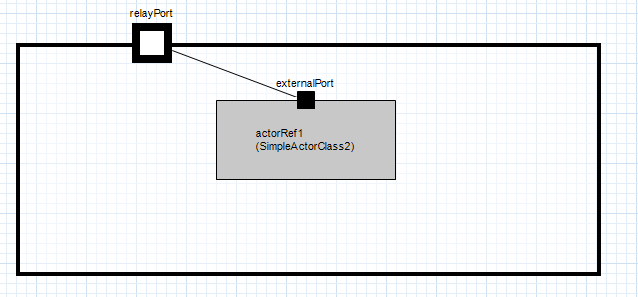
\includegraphics[scale=.7]{images/300-RelayPort.png}
		
		
		\begingroup
		\textbf{Features:}
		%\setlength{\tabcolsep}{10pt} % Default value: 6pt
		\renewcommand{\arraystretch}{1.8} % Default value: 1
		\begin{longtable}{l|l p{.5\textwidth}}
			\hline
		Is a: & \tabitem \hyperlink{ref:Port}{Port}  & A Port is an instance of a ProtocolClass and the interface for an ActorClass.\\
		\hline
		\end{longtable}
		\endgroup
		
		\begingroup
		\textbf{Feature Usage:}
		%\setlength{\tabcolsep}{10pt} % Default value: 6pt
		\renewcommand{\arraystretch}{1.8} % Default value: 1
		\begin{longtable}{l|l p{.5\textwidth}}
			\hline
		Is contained in: & \tabitem \hyperlink{ref:SubSystemClass}{SubSystemClass}  & The SubSystem is main Actor of an executable part of the system. \\
		\hline
		\end{longtable}
		\endgroup
		
		
	\vspace{\baselineskip}
	\vspace{\baselineskip}
	\vspace{\baselineskip}
	
	\subsubsection{SAP}
		\hypertarget{ref:SAP}{}
		
		A Service Access Point is similar to a Port, but uses a LayerConnection for wiring.
		
		\emph{\large Under construction}
		\begin{itemize}
		\item An actor class can define a Service Provision Point (SPP) to publish a specific service, defined by a protocol class
		\item An actor class can define a Service Access Point (SAP) if it needs a service, defined by a protocol class
		\item For a given actor hierarchy, a LayerConnection defines which SAP will be satisfied by (connected to) which SPP
		\end{itemize}
		
		
		\begingroup
		\textbf{Features:}
		%\setlength{\tabcolsep}{10pt} % Default value: 6pt
		\renewcommand{\arraystretch}{1.8} % Default value: 1
		\begin{longtable}{l|l p{.5\textwidth}}
			\hline
		Is of type: & \tabitem \hyperlink{ref:ProtocolClass}{ProtocolClass}  & A ProtocolClass defines messages and is the interface specification for a Port\\
		\hline
		\end{longtable}
		\endgroup
		
		\begingroup
		\textbf{Feature Usage:}
		%\setlength{\tabcolsep}{10pt} % Default value: 6pt
		\renewcommand{\arraystretch}{1.8} % Default value: 1
		\begin{longtable}{l|l p{.5\textwidth}}
			\hline
		Is contained in: & \tabitem \hyperlink{ref:ActorClass}{ActorClass}  & The actor is the basic structural building block for building systems with ROOM.\\
		\hline
		Is edited by: & \tabitem \hyperlink{ref:GraphicalStructureEditor}{GraphicalStructureEditor}  & The Structure Editor allows to edit the Actor Structure in a convenient way. It is possible to create and arrange actor references and ports and to create bindings and layer connections.\\
		\hline
		Is used by: & \tabitem \hyperlink{ref:LayerConnection}{LayerConnection} : SAPoint & A LayerConnection associates a SPP to an ActorRef, resulting in an connection of all SAPs on its instance hierarchy.\\
		\hline
		\end{longtable}
		\endgroup
		
		
	\vspace{\baselineskip}
	\vspace{\baselineskip}
	\vspace{\baselineskip}
	
	\subsubsection{SPP}
		\hypertarget{ref:SPP}{}
		
		A Service Provision Point is the counterpart of a SAP
		
		\emph{Under construction}
		\begin{itemize}
		\item An actor class can define a Service Provision Point (SPP) to publish a specific service, defined by a protocol class
		\item An actor class can define a Service Access Point (SAP) if it needs a service, defined by a protocol class
		\item For a given actor hierarchy, a LayerConnection defines which SAP will be satisfied by (connected to) which SPP
		\end{itemize}
		
		
		\begingroup
		\textbf{Features:}
		%\setlength{\tabcolsep}{10pt} % Default value: 6pt
		\renewcommand{\arraystretch}{1.8} % Default value: 1
		\begin{longtable}{l|l p{.5\textwidth}}
			\hline
		Is of type: & \tabitem \hyperlink{ref:ProtocolClass}{ProtocolClass}  & A ProtocolClass defines messages and is the interface specification for a Port\\
		\hline
		\end{longtable}
		\endgroup
		
		\begingroup
		\textbf{Feature Usage:}
		%\setlength{\tabcolsep}{10pt} % Default value: 6pt
		\renewcommand{\arraystretch}{1.8} % Default value: 1
		\begin{longtable}{l|l p{.5\textwidth}}
			\hline
		Is contained in: & \tabitem \hyperlink{ref:ActorClass}{ActorClass}  & The actor is the basic structural building block for building systems with ROOM.\\
		& \tabitem \hyperlink{ref:SubSystemClass}{SubSystemClass}  & The SubSystem is main Actor of an executable part of the system.  \\
		\hline
		Is edited by: & \tabitem \hyperlink{ref:SPPPropertyDialog}{SPPPropertyDialog}  & \\
		\hline
		Is used by: & \tabitem \hyperlink{ref:LayerConnection}{LayerConnection} : SPPoint & A LayerConnection associates a SPP to an ActorRef, resulting in an connection of all SAPs on its instance hierarchy.\\
		& \tabitem \hyperlink{ref:ServiceImplementation}{ServiceImplementation}  & The implementation of an Service Provision Point (SPP). \\
		\hline
		\end{longtable}
		\endgroup
		
		
	\vspace{\baselineskip}
	\vspace{\baselineskip}
	\vspace{\baselineskip}
	
	\subsubsection{StateMachine}
		\hypertarget{ref:StateMachine}{}
		
		A StateMachine describes the state based, event driven behavior of an ActorClass
		
		In ROOM each actor class can implement its behavior using a state machine. Events occurring at the end ports of an actor will be forwarded to and processed by the state machine. Events possibly trigger state transitions.
		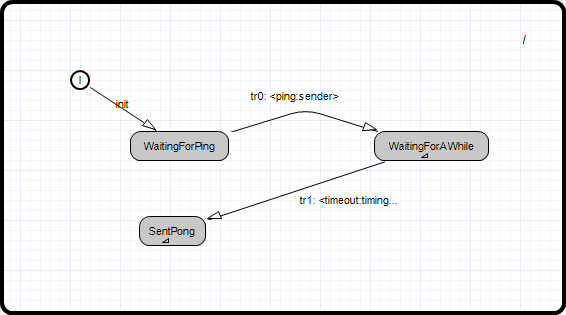
\includegraphics[scale=.7]{images/300-PingPongReceiverFSM.png}
		
		
		\begingroup
		\textbf{Features:}
		%\setlength{\tabcolsep}{10pt} % Default value: 6pt
		\renewcommand{\arraystretch}{1.8} % Default value: 1
		\begin{longtable}{l|l p{.5\textwidth}}
			\hline
		Uses: & \tabitem \hyperlink{ref:Inheritance}{Inheritance}  & A class can specify a super class and inherits elements from the super class hierarchy.\\
		\hline
		\end{longtable}
		\endgroup
		
		\begingroup
		\textbf{Feature Usage:}
		%\setlength{\tabcolsep}{10pt} % Default value: 6pt
		\renewcommand{\arraystretch}{1.8} % Default value: 1
		\begin{longtable}{l|l p{.5\textwidth}}
			\hline
		Is contained in: & \tabitem \hyperlink{ref:ActorClass}{ActorClass}  & The actor is the basic structural building block for building systems with ROOM.\\
		\hline
		\end{longtable}
		\endgroup
		
		
	\vspace{\baselineskip}
	\vspace{\baselineskip}
	\vspace{\baselineskip}
	
	\subsubsection{SubSystemClass}
		\hypertarget{ref:SubSystemClass}{}
		
		The SubSystem is main Actor of an executable part of the system. 
		
		It instantiates the Actor instance tree instance of the application ...
		
		Actor instance tree example:
		
		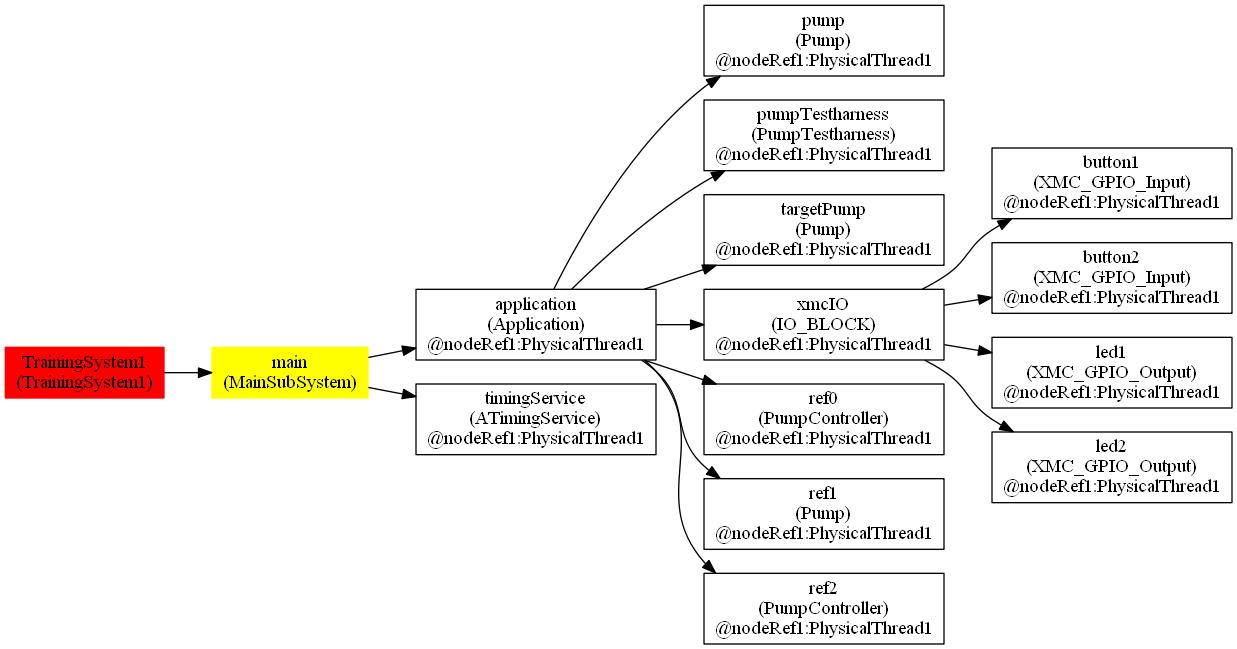
\includegraphics[width=\textwidth]{images/300-TrainingSystem1_instanceTree.jpg}
		
		
		\begingroup
		\textbf{Features:}
		%\setlength{\tabcolsep}{10pt} % Default value: 6pt
		\renewcommand{\arraystretch}{1.8} % Default value: 1
		\begin{longtable}{l|l p{.5\textwidth}}
			\hline
		Contains: & \tabitem \hyperlink{ref:ActorRef}{ActorRef}  & An ActorRef is an instance of an ActorClass.\\
		& \tabitem \hyperlink{ref:RelayPort}{RelayPort}  & A RelayPort forwards its messages without exposing them to the internal interface of the ActorClass. \\
		& \tabitem \hyperlink{ref:SPP}{SPP}  & A Service Provision Point is the counterpart of a SAP \\
		& \tabitem \hyperlink{ref:Binding}{Binding}  & A Binding connects two Ports with each other. \\
		& \tabitem \hyperlink{ref:LayerConnection}{LayerConnection}  & A LayerConnection associates a SPP to an ActorRef, resulting in an connection of all SAPs on its instance hierarchy. \\
		\hline
		\end{longtable}
		\endgroup
		
		\begingroup
		\textbf{Feature Usage:}
		%\setlength{\tabcolsep}{10pt} % Default value: 6pt
		\renewcommand{\arraystretch}{1.8} % Default value: 1
		\begin{longtable}{l|l p{.5\textwidth}}
			\hline
		Typecasts: & \tabitem \hyperlink{ref:SubSystemRef}{SubSystemRef}  & A Sub System Reference is an instance of an SubSystemClass\\
		\hline
		Is contained in: & \tabitem \hyperlink{ref:LogicalModel}{LogicalModel}  & The LogicalModel describes the logical structure and behavior of a ROOM application.\\
		\hline
		\end{longtable}
		\endgroup
		
		
	\vspace{\baselineskip}
	\vspace{\baselineskip}
	\vspace{\baselineskip}
	
	\subsubsection{SubSystemRef}
		\hypertarget{ref:SubSystemRef}{}
		
		A Sub System Reference is an instance of an SubSystemClass
		
		
		
		\begingroup
		\textbf{Features:}
		%\setlength{\tabcolsep}{10pt} % Default value: 6pt
		\renewcommand{\arraystretch}{1.8} % Default value: 1
		\begin{longtable}{l|l p{.5\textwidth}}
			\hline
		Is of type: & \tabitem \hyperlink{ref:SubSystemClass}{SubSystemClass}  & The SubSystem is main Actor of an executable part of the system. \\
		\hline
		\end{longtable}
		\endgroup
		
		\begingroup
		\textbf{Feature Usage:}
		%\setlength{\tabcolsep}{10pt} % Default value: 6pt
		\renewcommand{\arraystretch}{1.8} % Default value: 1
		\begin{longtable}{l|l p{.5\textwidth}}
			\hline
		Is contained in: & \tabitem \hyperlink{ref:LogicalSystem}{LogicalSystem}  & The top level structural class. It can only contain sub systems using SubSystemRefs.\\
		\hline
		\end{longtable}
		\endgroup
		
		
	\vspace{\baselineskip}
	\vspace{\baselineskip}
	\vspace{\baselineskip}
	\subsection{PhysicalModel}
	The PhysicalModel describes the topology of the targets a distributed system can be deployed (mapped) on.
	
	
	
	\subsection{MappingModel}
	The MappingModel describes the mapping of elements of the LogicalModel to elements of the PhysicalModel.
	
	It enables the complete decoupling of the LogicalModel and the PhysicalModel, thus providing a maximum flexibility and reuse for the models.
	
	\begingroup
	\textbf{Features:}
	%\setlength{\tabcolsep}{10pt} % Default value: 6pt
	\renewcommand{\arraystretch}{1.8} % Default value: 1
	\begin{longtable}{l|l p{.5\textwidth}}
		\hline
	Uses: & \tabitem \hyperlink{ref:LogicalModel}{LogicalModel}  & The LogicalModel describes the logical structure and behavior of a ROOM application.\\
	& \tabitem \hyperlink{ref:PhysicalModel}{PhysicalModel}  & The PhysicalModel describes the topology of the targets a distributed system can be deployed (mapped) on. \\
	\hline
	\end{longtable}
	\endgroup
	
	\subsection{ConfigModel}
	The ConfigModel describes the Attribute configuration of ActorInstances and PortInstances. 
	
	
	
\section{ModelEditors}
	
	
	\subsection{TextualROOMEditor}
	Textual model editor
	
	
	\begingroup
	\textbf{Features:}
	%\setlength{\tabcolsep}{10pt} % Default value: 6pt
	\renewcommand{\arraystretch}{1.8} % Default value: 1
	\begin{longtable}{l|l p{.5\textwidth}}
		\hline
	Is a: & \tabitem \hyperlink{ref:ModelEditor}{ModelEditor}  & ModelEditor\\
	\hline
	\end{longtable}
	\endgroup
	
	\subsection{GraphicalStructureEditor}
	The Structure Editor allows to edit the Actor Structure in a convenient way. It is possible to create and arrange actor references and ports and to create bindings and layer connections.
	
	
	\begingroup
	\textbf{Features:}
	%\setlength{\tabcolsep}{10pt} % Default value: 6pt
	\renewcommand{\arraystretch}{1.8} % Default value: 1
	\begin{longtable}{l|l p{.5\textwidth}}
		\hline
	Is a: & \tabitem \hyperlink{ref:ModelEditor}{ModelEditor}  & ModelEditor\\
	\hline
	Contains: & \tabitem \hyperlink{ref:StructureEditiorPalette}{StructureEditiorPalette}  & creates all Kinds of ...  picture with explanation\\
	& \tabitem \hyperlink{ref:ActorRefPropertyDialog}{ActorRefPropertyDialog}  & A Dialog to edit structural reference of an ActorRef.
	 \\
	& \tabitem \hyperlink{ref:PortPropertyDialog}{PortPropertyDialog}  &  \\
	& \tabitem \hyperlink{ref:SPPPropertyDialog}{SPPPropertyDialog}  &  \\
	\hline
	Edits: & \tabitem \hyperlink{ref:ActorClass}{ActorClass}  & The actor is the basic structural building block for building systems with ROOM.\\
	& \tabitem \hyperlink{ref:ActorRef}{ActorRef}  & An ActorRef is an instance of an ActorClass. \\
	& \tabitem \hyperlink{ref:Port}{Port}  & A Port is an instance of a ProtocolClass and the interface for an ActorClass. \\
	& \tabitem \hyperlink{ref:SAP}{SAP}  & A Service Access Point is similar to a Port, but uses a LayerConnection for wiring. \\
	& \tabitem \hyperlink{ref:Binding}{Binding}  & A Binding connects two Ports with each other. \\
	& \tabitem \hyperlink{ref:LayerConnection}{LayerConnection}  & A LayerConnection associates a SPP to an ActorRef, resulting in an connection of all SAPs on its instance hierarchy. \\
	\hline
	\end{longtable}
	\endgroup
	
	
	\subsubsection{ActorRefPropertyDialog}
		\hypertarget{ref:ActorRefPropertyDialog}{}
		
		A Dialog to edit structural reference of an ActorRef.
		
		
		
		\begingroup
		\textbf{Features:}
		%\setlength{\tabcolsep}{10pt} % Default value: 6pt
		\renewcommand{\arraystretch}{1.8} % Default value: 1
		\begin{longtable}{l|l p{.5\textwidth}}
			\hline
		Edits: & \tabitem \hyperlink{ref:ActorRef}{ActorRef}  & An ActorRef is an instance of an ActorClass.\\
		\hline
		\end{longtable}
		\endgroup
		
		\begingroup
		\textbf{Feature Usage:}
		%\setlength{\tabcolsep}{10pt} % Default value: 6pt
		\renewcommand{\arraystretch}{1.8} % Default value: 1
		\begin{longtable}{l|l p{.5\textwidth}}
			\hline
		Is contained in: & \tabitem \hyperlink{ref:GraphicalStructureEditor}{GraphicalStructureEditor}  & The Structure Editor allows to edit the Actor Structure in a convenient way. It is possible to create and arrange actor references and ports and to create bindings and layer connections.\\
		\hline
		\end{longtable}
		\endgroup
		
		
	\vspace{\baselineskip}
	\vspace{\baselineskip}
	\vspace{\baselineskip}
	
	\subsubsection{PortPropertyDialog}
		\hypertarget{ref:PortPropertyDialog}{}
		
		
		
		
		\begingroup
		\textbf{Features:}
		%\setlength{\tabcolsep}{10pt} % Default value: 6pt
		\renewcommand{\arraystretch}{1.8} % Default value: 1
		\begin{longtable}{l|l p{.5\textwidth}}
			\hline
		Edits: & \tabitem \hyperlink{ref:Port}{Port}  & A Port is an instance of a ProtocolClass and the interface for an ActorClass.\\
		\hline
		\end{longtable}
		\endgroup
		
		\begingroup
		\textbf{Feature Usage:}
		%\setlength{\tabcolsep}{10pt} % Default value: 6pt
		\renewcommand{\arraystretch}{1.8} % Default value: 1
		\begin{longtable}{l|l p{.5\textwidth}}
			\hline
		Is contained in: & \tabitem \hyperlink{ref:GraphicalStructureEditor}{GraphicalStructureEditor}  & The Structure Editor allows to edit the Actor Structure in a convenient way. It is possible to create and arrange actor references and ports and to create bindings and layer connections.\\
		\hline
		\end{longtable}
		\endgroup
		
		
	\vspace{\baselineskip}
	\vspace{\baselineskip}
	\vspace{\baselineskip}
	
	\subsubsection{SPPPropertyDialog}
		\hypertarget{ref:SPPPropertyDialog}{}
		
		
		
		
		\begingroup
		\textbf{Features:}
		%\setlength{\tabcolsep}{10pt} % Default value: 6pt
		\renewcommand{\arraystretch}{1.8} % Default value: 1
		\begin{longtable}{l|l p{.5\textwidth}}
			\hline
		Edits: & \tabitem \hyperlink{ref:SPP}{SPP}  & A Service Provision Point is the counterpart of a SAP\\
		\hline
		\end{longtable}
		\endgroup
		
		\begingroup
		\textbf{Feature Usage:}
		%\setlength{\tabcolsep}{10pt} % Default value: 6pt
		\renewcommand{\arraystretch}{1.8} % Default value: 1
		\begin{longtable}{l|l p{.5\textwidth}}
			\hline
		Is contained in: & \tabitem \hyperlink{ref:GraphicalStructureEditor}{GraphicalStructureEditor}  & The Structure Editor allows to edit the Actor Structure in a convenient way. It is possible to create and arrange actor references and ports and to create bindings and layer connections.\\
		\hline
		\end{longtable}
		\endgroup
		
		
	\vspace{\baselineskip}
	\vspace{\baselineskip}
	\vspace{\baselineskip}
	
	\subsubsection{StructureEditiorPalette}
		\hypertarget{ref:StructureEditiorPalette}{}
		
		creates all Kinds of ...  picture with explanation
		
		
		
		
		\begingroup
		\textbf{Feature Usage:}
		%\setlength{\tabcolsep}{10pt} % Default value: 6pt
		\renewcommand{\arraystretch}{1.8} % Default value: 1
		\begin{longtable}{l|l p{.5\textwidth}}
			\hline
		Is contained in: & \tabitem \hyperlink{ref:GraphicalStructureEditor}{GraphicalStructureEditor}  & The Structure Editor allows to edit the Actor Structure in a convenient way. It is possible to create and arrange actor references and ports and to create bindings and layer connections.\\
		\hline
		\end{longtable}
		\endgroup
		
		
	\vspace{\baselineskip}
	\vspace{\baselineskip}
	\vspace{\baselineskip}
	\subsection{GraphicalBehaviorEditor}
	ModelEditor
	
	
	\begingroup
	\textbf{Features:}
	%\setlength{\tabcolsep}{10pt} % Default value: 6pt
	\renewcommand{\arraystretch}{1.8} % Default value: 1
	\begin{longtable}{l|l p{.5\textwidth}}
		\hline
	Is a: & \tabitem \hyperlink{ref:ModelEditor}{ModelEditor}  & ModelEditor\\
	\hline
	\end{longtable}
	\endgroup
	
\section{CodeGenerators}
	
	
	\subsection{CCodeGenerator}
	
	
	\begingroup
	\textbf{Features:}
	%\setlength{\tabcolsep}{10pt} % Default value: 6pt
	\renewcommand{\arraystretch}{1.8} % Default value: 1
	\begin{longtable}{l|l p{.5\textwidth}}
		\hline
	Is a: & \tabitem \hyperlink{ref:CodeGenerator}{CodeGenerator}  & \\
	\hline
	\end{longtable}
	\endgroup
	
	\subsection{JavaCodeGenerator}
	
	
	\begingroup
	\textbf{Features:}
	%\setlength{\tabcolsep}{10pt} % Default value: 6pt
	\renewcommand{\arraystretch}{1.8} % Default value: 1
	\begin{longtable}{l|l p{.5\textwidth}}
		\hline
	Is a: & \tabitem \hyperlink{ref:CodeGenerator}{CodeGenerator}  & \\
	\hline
	\end{longtable}
	\endgroup
	

